\chapter{Проектування програмних засобів}
В цьому розділі будуть сформульовані вимоги до програмного середовища, в якому необхідно реалізувати метод пошуку
шаблонів за допомогою поліномів Кунченко.
Будуть наведені можливі варіанти вибору й обґрунтований вибір.
Буде спроектована архітектура програмної реалізації та наведений алгоритм роботи цієї реалізації.

\section{Вибір програмного середовища}
    Для полегшення розробки та забезпечення високої якості роботи програмних засобів, було вирішено використати один з
    існуючих математичних пакетів для роботи з цифровими сигналами.

    Серед інших, розглядалися наступні математичні пакети: Mathworks\textsuperscript{\textregistered}
    MATLAB\textsuperscript{\textregistered} 2014b, GNU Octave, Python+Numpy.
    Порівняльна характеристика цих пакетів наведена в таблиці~\ref{tab:math}.

    \stepcounter{tablecount}
    \begin{table}
        {|p{0.1\textwidth}|C{0.3\textwidth}|C{0.27\textwidth}|p{0.15\textwidth}|}
        {Порівняльна характеристика математичних пакетів}
        {tab:math}
        {\hline
            & Кросплатформенність & Мінімальний розмір & Ліцензія\\
            \hline}
        Matlab & + & 1200 МіБ & Propr.\\
        Octave & + & 650 МіБ  & GPL\\
        Numpy  & + & 112 МіБ  & BSD-new\\
    \end{table}

    Усі ці середовища зарекомендували себе як якісне математичне забезпечення для обробки сигналів.

    Matlab є найстарішим математичним пакетом із пакетів, що розглядалися.
    Для цієї середи було написано безліч модулів для обробки сигналів і не тільки.
    Також, із усіх пакетів, що розглядалися, тільки в цьому пакеті є вбудована можливість апаратного прискорення
    обчислень на відеочіпі, що дає значний приріст продуктивності при обробці цифрових сигналів.

    Середовище Octave було розроблено як альтернатива Matlab.
    Воно підтримує синтаксис вбудованої мови Matlab, і саме тому безліч модулів, що були написані для Matlab, працюють
    і на Octave.
    Цей пакет є програмним забезпеченням із відкритим кодом, що є значною перевагою над Matlab.
    Також варто зазначити, що цей пакет розвивається набагато швидше за Matlab, а тому, можливо, в майбутньому в ньому
    будуть функції, що зараз є лише в Matlab (наприклад, апаратне прискорення обчислень).

    Numpy, на відміну від Matlab та Octave, є набором модулів/бібліотек для мови програмування Python.
    З усіх систем, Numpy розвивається найактивніше.
    До переваг Numpy можна віднести те, що програми на Numpy --- це програми на мові Python, яка є набагато
    поширенішою за мови Matlab/Octave.
    Також ліцензія, за якою розповсюджується Numpy є більш вільною за GPL (за якою розповсюджується Octave), що
    дозволяє використовувати це середовище для комерційної розробки.

    Для початкового проектування й дослідження було обрано середовище Matlab, оскільки знайти необхідний модуль для
    цього середовища значно легше, а можливість використовувати апаратне прискорення також є дуже бажаною
    характеристикою.
\section{Проектування архітектури програмної реалізації}
    Оскільки було обрано математичне середовище Matlab, програмна реалізація методу пошуку шаблонів за допомогою
    розкладення функції поліномами Кунченка складається із наступних функцій"=скриптів:
    \begin{itemize}
        \item \verb'match' --- функція"=інтерфейс, точка входу до модуля пошуку шаблонів.
            Отримує параметрами цифровий сигнал, шаблон, функціональні перетворення, за допомогою яких будується
            лінійний простір над породжуючою функцією.
            Саме в цій функції виконується \invcommas{ковзання} вікна.
            Ця функція, в свою чергу, викликає \verb'buildGeneratedFunctionsSystem', \verb'createIterator',
            \verb'approximate'.
        \item \verb'buildGeneratedFunctionsSystem' --- функція, що будує базиси лінійного простору Кунченко та
            обчислює центровані скалярні добутки між ними.
        \item \verb'createIterator' --- створює вікно й дозволяє рухати це вікно заданим чином.
        \item \verb'approximate' --- обчислює апроксимацію обраного вікна вхідного сигналу базисом лінійного простору
            Кунченко.
            В цій функції будується система лінійних рівнянь, з якої знаходяться коефіцієнти при базисних функціях
            лінійного простору, рахується коефіцієнт наближення вхідного сигналу за допомогою породжених функцій.
    \end{itemize}

    Таким чином було створено наступні рівні абстракції:
    \begin{itemize}
        \item Базис лінійного простору, що містить наступні поля:
            \begin{itemize}
                \item породжуюча функція (шаблон);
                \item породжені функції (функціональні перетворення шаблону);
                \item посилання на функцію скалярного добутку;
                \item наперед підраховані значення скалярного добутку для усіх пар породжених функцій.
            \end{itemize}

            Посилання на функцію скалярного добутку в цій структурі дозволяє змінювати метод пошуку корелянти між
            двома функціями.
            За замовчанням це є чисельне інтегрування методом трапецій від попарного добутку значень аргументів.
        \item Ітератор в сигналі, який дозволяє певним чином обходити довільний сигнал.
            Змінюючи реалізацію цього ітератору можна змінювати вигляд вікна вхідного сигналу, змінювати шаг між
            вікнами тощо.
    \end{itemize}

\section{Алгоритм роботи програми}
На рисунку~\ref{fig:block_scheme_monitor} наведено блок"=схему алгоритму пошуку шаблонів.
    \stepcounter{figurecount}
    \begin{figure}[h]
        \centering
        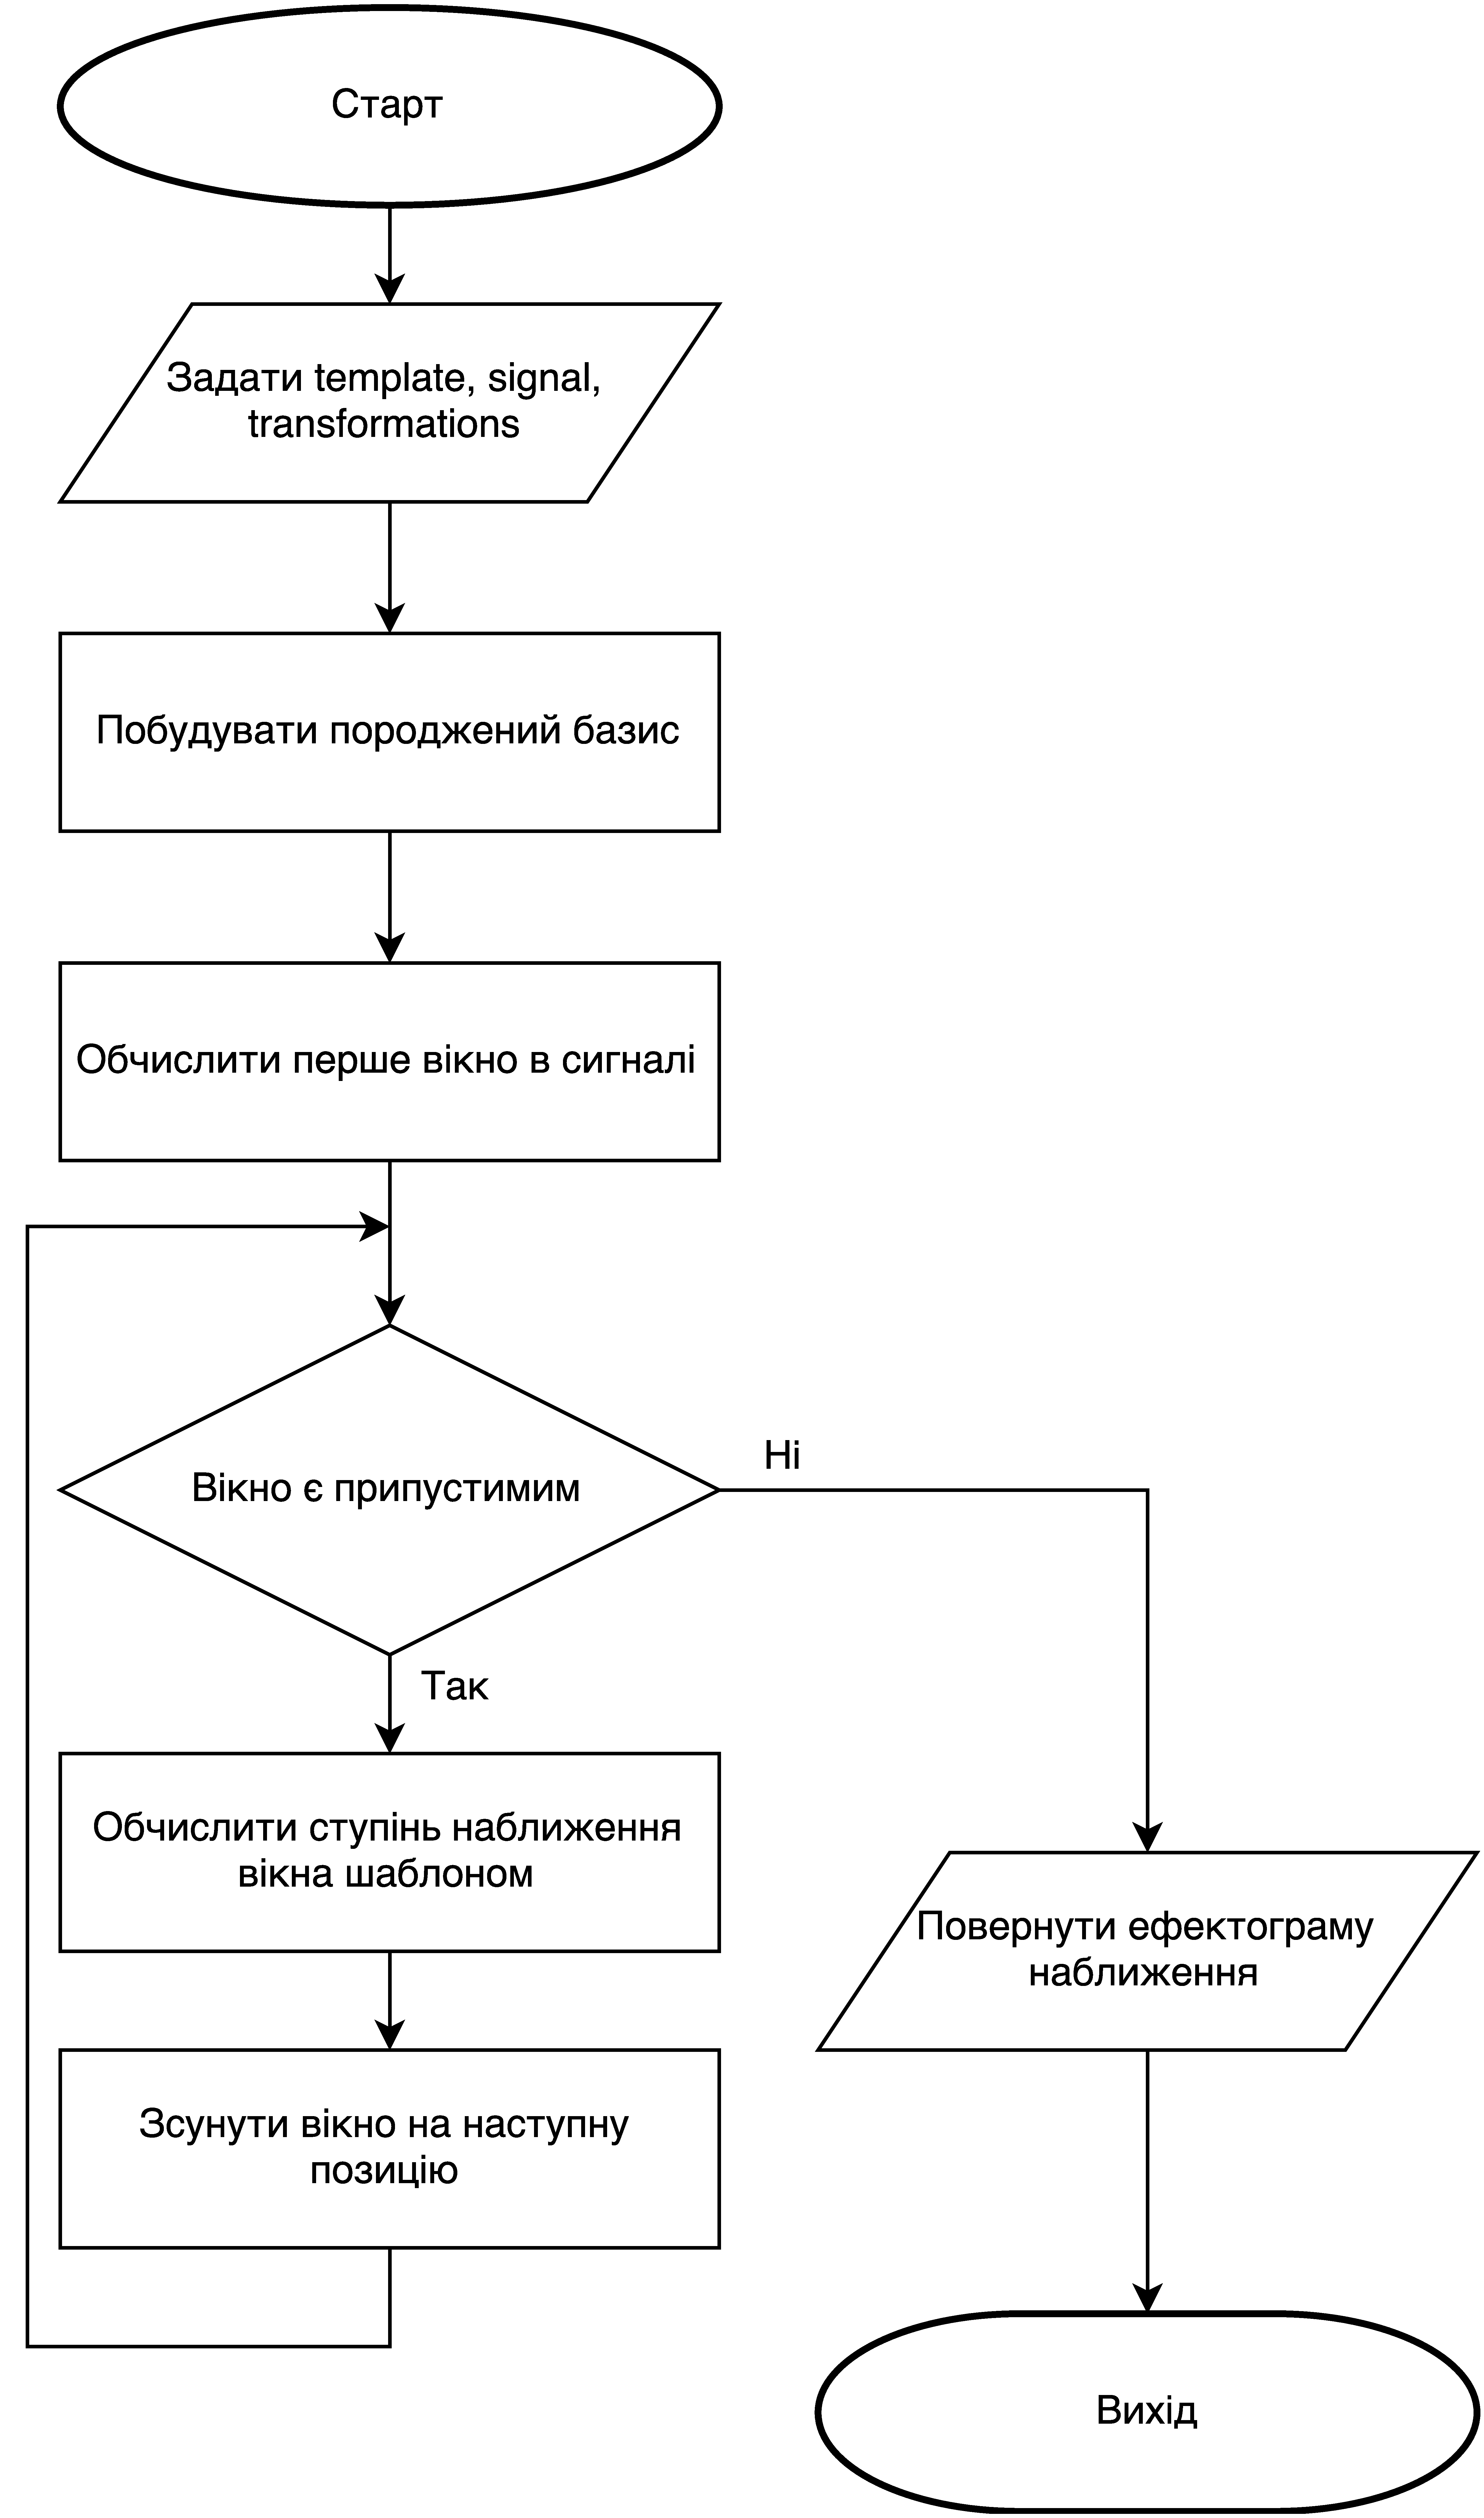
\includegraphics[height=0.72\textheight]{Drawing2.eps}
        \caption{Блок"=схема роботи алгоритму пошуку шаблону}
        \label{fig:block_scheme_monitor}
    \end{figure}
    \clearpage

\section{Висновки}
    В цьому розділі було обґрунтовано вибір середовища Matlab як середовища з великою кількістю модулів для обробки
    цифрових сигналів.

    Завдяки абстрагуванню спроектована система має достатню гнучкість, щоб змінювати метод пошуку наступного вікна та
    обчислення скалярного добутку.
    Завдяки цьому отримана система дозволяє шукати шаблон не лише в одновимірному сигналі, а й в двовимірному.

    Також можна зазначити, що після дослідження методу пошуку шаблонів за допомогою розкладення функції в лінійному
    просторі Кунченка, систему можна буде перевести в середовище Numpy, щоб можна було користуватися багатьма
    системними бібліотеками, що розроблені для мови програмування Python.
    Це дозволить програмному продукту мати, наприклад, графічний інтерфейс користувача.

    Також має сенс мати сумісність з математичним середовищем Octave, адже останнє, на відміну від Matlab, є
    безкоштовним ПЗ з відкритим вихідним кодом.

% vim: spelllang=uk,en spell filetype=tex

